\section{Auswertung}
\label{sec:Auswertung}

%\begin{figure}
%  \centering
%  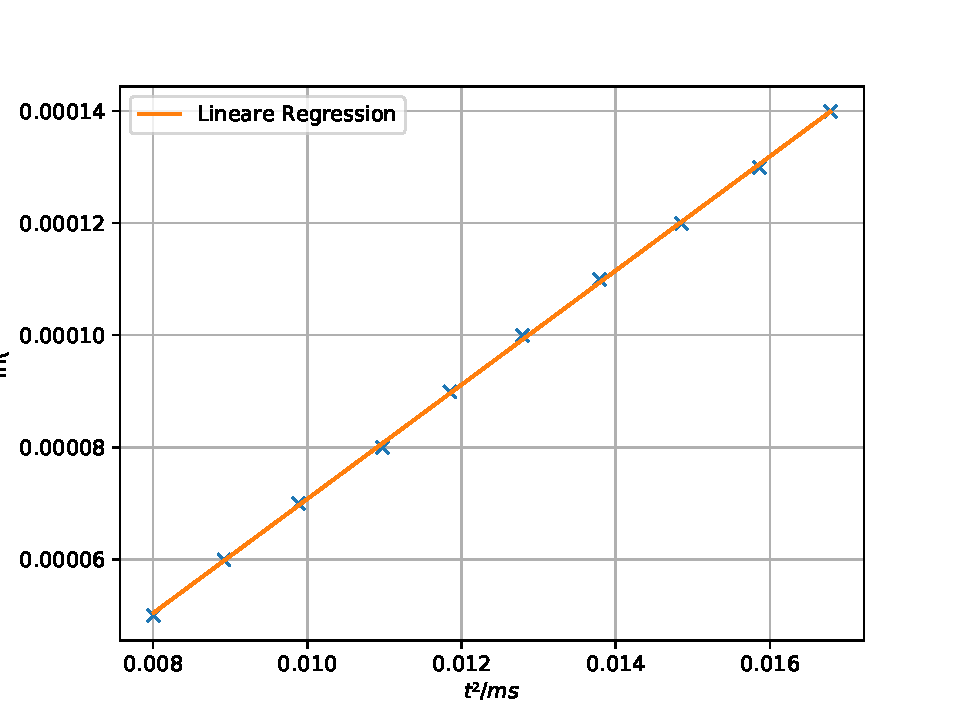
\includegraphics{Graphibitte.pdf}
%  \caption{Plot.}
%  \label{fig:plot}
%\end{figure}

%Einheiten: \SI{3}{\newton\s}
%1,41 \cdot \cramped{10^{-3}} ~s  für hochzahlen

%\begin{table}
%  \centering
%  \caption{Tabelle für a)Erste Bestimmung der Zeitkonstanten}
%  \label{Tab1}
%    \begin{tabular}{c c}%c zeigt die anzahl der Spalten
%      \toprule
%      Spannung $U_c$ &Zeit $t$\\% \\ werden benötigt um die Zeile zu Beenden
%      mV&ms\\% & Zeichen grenzen die Zahlen voneinander ab.
%      \midrule
%      \midrule
%        %\input{tab1.txt}% Die Tabelle ist hier ausgelagert. Sie kann aber auch genausogut hier eingefügt werden.
%          0,000 &     752\\
%          0,400 &     440\\
%          0,800 &     448\\
%      \bottomrule
%    \end{tabular}
%\end{table}

%\begin{table}
%    \centering
%    \caption{Messwerte für die Beta-Strahlung.}
%    \label{Tabg}
%    \sisetup{table-format=1.2}
%    \begin{tabular}{S S[table-format=2.2] S } %3 ziffern vom kommer, zwei danach, geht hiter jedes s
%      \toprule
%      %{$D$/cm}& \multicolumn{5}{c}{$U_{\symup{B}i} = \,\si{V}$}\\ überschrift über mehrere spalten
%      %\midrule
%       {$D/ \mu\si{m}$}& {$R/\frac{\si{kg}}{\si{m²}}$} & {$t$/s} &  {$N$} & {$A_{\symup{gem}} = \frac{N}{t}/ \frac{1}{\si{s}}$}  & {$A/ \frac{1}{\si{s}}$}  & {$\symup{ln}(A)$}\\
%      \midrule
%      \midrule
%          {$ 3924 \pm 62$} & 39,24 & {$ ~~3,652 \pm 0,016$}\\
%          {$ 2122 \pm 46$} & 10,61 & {$ ~~2,296 \pm 0,023$}\\
%          {$ 3001 \pm 54$} & 10,00 & {$ ~~2,233 \pm 0,019$}\\
%      \bottomrule
%    \end{tabular}
%\end{table}

%Mittelwert von X:
%\begin{equation*}
%  \overline{X }=  \frac{1}{N} \sum_{i=1}^N (X_i) = 75,98 \, \si{Hz} 
%\end{equation*}
%Formel für den Fehler des Mittelwerts:
%\begin{equation*}
%  \symup{\Delta} X = \frac{1}{\sqrt{N}} \sqrt{\frac{1}{\sqrt{N-1}} \sum_{i=1}^N (X_{i}-\overline{X})²}= 0,02 \, \si{Hz} 
%\end{equation*}

\begin{table}
    \centering
    \caption{Messwerte für die Wärmekapazitätsberechnung.}
    \label{Tabg}
    \sisetup{table-format=1.2}
    \begin{tabular}{S[table-format=2.1] S S[table-format=2.1] S S} %3 ziffern vom kommer, zwei danach, geht hiter jedes s
      \toprule
      %{$D$/cm}& \multicolumn{5}{c}{$U_{\symup{B}i} = \,\si{V}$}\\ überschrift über mehrere spalten
      %\midrule
       {$U/ \si{V}$}& {$I/\si{mA}$} & {$t$/s} & {$T$/K} & {$\symup{\Delta}T$/K}\\
      \midrule
      \midrule
          {16,69} & {160,3}  &  9,5 & -180,1 & {$274$}  \\
          {16,95} & {161,2}  & 10,2 & -169,8 & {$320$}  \\
          {17,05} & {162,0}  & 10,0 & -159,8 & {$335$}  \\
          {17,15} & {162,8}  & 10,1 & -149,8 & {$369$}  \\
          {18,80} & {178,0}  &  9,9 & -139,9 & {$309$}  \\
          {18,65} & {176,8}  &  9,9 & -130,2 & {$329$}  \\
          {19,79} & {187,4}  & 10,0 & -120,0 & {$307$}  \\
          {19,86} & {188,0}  & 10,0 & -110,0 & {$307$}  \\
          {19,90} & {188,3}  & 10,1 &  -99,9 & {$310$}  \\
          {19,93} & {188,5}  & 10,1 &  -89,8 & {$317$}  \\
          {19,96} & {188,7}  &  9,9 &  -80,0 & {$322$}  \\
          {19,98} & {188,9}  &  9,9 &  -70,0 & {$326$}  \\
          {20,0 } & {189,1}  & 10,0 &  -60,0 & {$324$}  \\
          {20,0 } & {189,2}  & 10,0 &  -50,0 & {$300$}  \\
          {20,1 } & {189,3}  &  9,8 &  -40,2 & {$379$}  \\
          {20,0 } & {189,4}  & 10,1 &  -30,2 & {$367$}  \\
          {20,0 } & {189,5}  &  9,9 &  -20,2 & {$266$}  \\
          {20,0 } & {189,5}  & 10,2 &  -10,0 & {$367$}  \\
          {20,0 } & {189,6}  & 10,0 &    0,0 & {$371$}  \\
          {20,0 } & {189,6}  & 10,0 &   10,0 & {$383$}  \\
          {20,0 } & {189,7}  & 10,1 &   20,1 & {$375$}  \\
          {20,0 } & {189,8}  & 10,1 &   30,2 & {$375$}  \\
      \bottomrule
    \end{tabular}
\end{table}

 
  
  
 
  
  
  
 
  
  
 
 
  
  
  
 
  
 
 
 
 
 